% $Header: /cvsroot/latex-beamer/latex-beamer/solutions/conference-talks/conference-ornate-20min.en.tex,v 1.6 2004/10/07 20:53:08 tantau Exp $

\documentclass{beamer}
%\documentclass[handout]{beamer}
%\usepackage{pgfpages}
%\pgfpagesuselayout{2 on 1}[a4paper,border shrink=5mm]

% This file is a solution template for:

% - Talk at a conference/colloquium.
% - Talk length is about 20min.
% - Style is ornate.



% Copyright 2004 by Till Tantau <tantau@users.sourceforge.net>.
%
% In principle, this file can be redistributed and/or modified under
% the terms of the GNU Public License, version 2.
%
% However, this file is supposed to be a template to be modified
% for your own needs. For this reason, if you use this file as a
% template and not specifically distribute it as part of a another
% package/program, I grant the extra permission to freely copy and
% modify this file as you see fit and even to delete this copyright
% notice.


\mode<presentation>
{
%  \usetheme{Warsaw}
%  \usetheme{Boadilla}
%  \usetheme{Goettingen}
%  \usetheme{Hannover}
%  \usetheme{Madrid}
%  \usetheme{Marburg}
%  \usetheme{Montpellier}
%  \usetheme{Pittsburgh}
  \usetheme{Hawke}
  % or ...

  \setbeamercovered{transparent}
  % or whatever (possibly just delete it)
}


\usepackage[english]{babel}
% or whatever

\usepackage[latin1]{inputenc}
% or whatever

\usepackage{times}
\usepackage[T1]{fontenc}
% Or whatever. Note that the encoding and the font should match. If T1
% does not look nice, try deleting the line with the fontenc.

\usepackage{multimedia}


%%%%%%
% My Commands
%%%%%%

\newcommand{\ml}{{\sc matlab}}
\newcommand{\bb}{{\boldsymbol{b}}}
\newcommand{\bx}{{\boldsymbol{x}}}
\newcommand{\by}{{\boldsymbol{y}}}
\newcommand{\bfm}[1]{{\boldsymbol{#1}}}

%%%%

\title[Lecture 20] % (optional, use only with long paper titles)
{Lecture 20 - Stability of Multistep Methods}

% \subtitle
% {Include Only If Paper Has a Subtitle}

\author[I. Hawke] % (optional, use only with lots of authors)
{I.~Hawke}
% - Give the names in the same order as the appear in the paper.
% - Use the \inst{?} command only if the authors have different
%   affiliation.

\institute[University of Southampton] % (optional, but mostly needed)
{
%  \inst{1}%
  School of Mathematics, \\
  University of Southampton, UK
}
% - Use the \inst command only if there are several affiliations.
% - Keep it simple, no one is interested in your street address.

\date[Semester 1] % (optional, should be abbreviation of conference name)
{MATH3018/6141, Semester 1}
% - Either use conference name or its abbreviation.
% - Not really informative to the audience, more for people (including
%   yourself) who are reading the slides online

\subject{Numerical methods}
% This is only inserted into the PDF information catalog. Can be left
% out.



% If you have a file called "university-logo-filename.xxx", where xxx
% is a graphic format that can be processed by latex or pdflatex,
% resp., then you can add a logo as follows:

\pgfdeclareimage[height=0.5cm]{university-logo}{mathematics_7469}
\logo{\pgfuseimage{university-logo}}



% Delete this, if you do not want the table of contents to pop up at
% the beginning of each subsection:
%  \AtBeginSubsection[]
%  {
%    \begin{frame}<beamer>
%      \frametitle{Outline}
%      \tableofcontents[currentsection,currentsubsection]
%    \end{frame}
%  }
\AtBeginSection[]
{
  \begin{frame}<beamer>
    \frametitle{Outline}
    \tableofcontents[currentsection]
  \end{frame}
}


% If you wish to uncover everything in a step-wise fashion, uncomment
% the following command:

%\beamerdefaultoverlayspecification{<+->}


\begin{document}

\begin{frame}
  \titlepage
\end{frame}

\section{Stability of Multistep Methods}

\subsection{Stability of Multistep Methods}

\begin{frame}
  \frametitle{Multistep Methods}

  Looking at IVPs of the form
  \begin{equation*}
    \by'(x) = \bfm{f}(x, \by(x)).
  \end{equation*} \pause

  Looked at the multistep methods using the $k$-step method formula
  \begin{equation*}
    a_k y_{n+1} + a_{k-1} y_n + \dots + a_0 y_{n+1-k} = h \left[ b_k
      f_{n+1} + b_{k-1} f_n + \dots + b_0 f_{n+1-k} \right];
  \end{equation*}
  explicit when $b_k = 0$, implicit otherwise. All multistep methods
  need a different method to start. \pause

  \vspace{1ex}

  Under what circumstances do we get the right results?

\end{frame}

\begin{frame}
  \frametitle{Example}


  \begin{columns}
    \begin{column}{0.5\textwidth}
      Integrate
      \begin{equation*}
        y'(x) = -y, \quad y(0) = 1
      \end{equation*}
      with solution $y = \exp(- y(0) x)$. \pause

      \vspace{1ex}

      Using Milne's method the result diverges in an oscillatory
      fashion. \pause

      \vspace{1ex}

      Improve step size ($h = 0.01 \rightarrow 0.001$) just delays the
      oscillations. \pause

      \vspace{1ex}

      Contrast with Adams-Bashforth 5, which is fine.
    \end{column}
    \begin{column}{0.5\textwidth}
      \begin{overlayarea}{\textwidth}{0.6\textheight}
        \only<2>
        {
          \begin{center}
            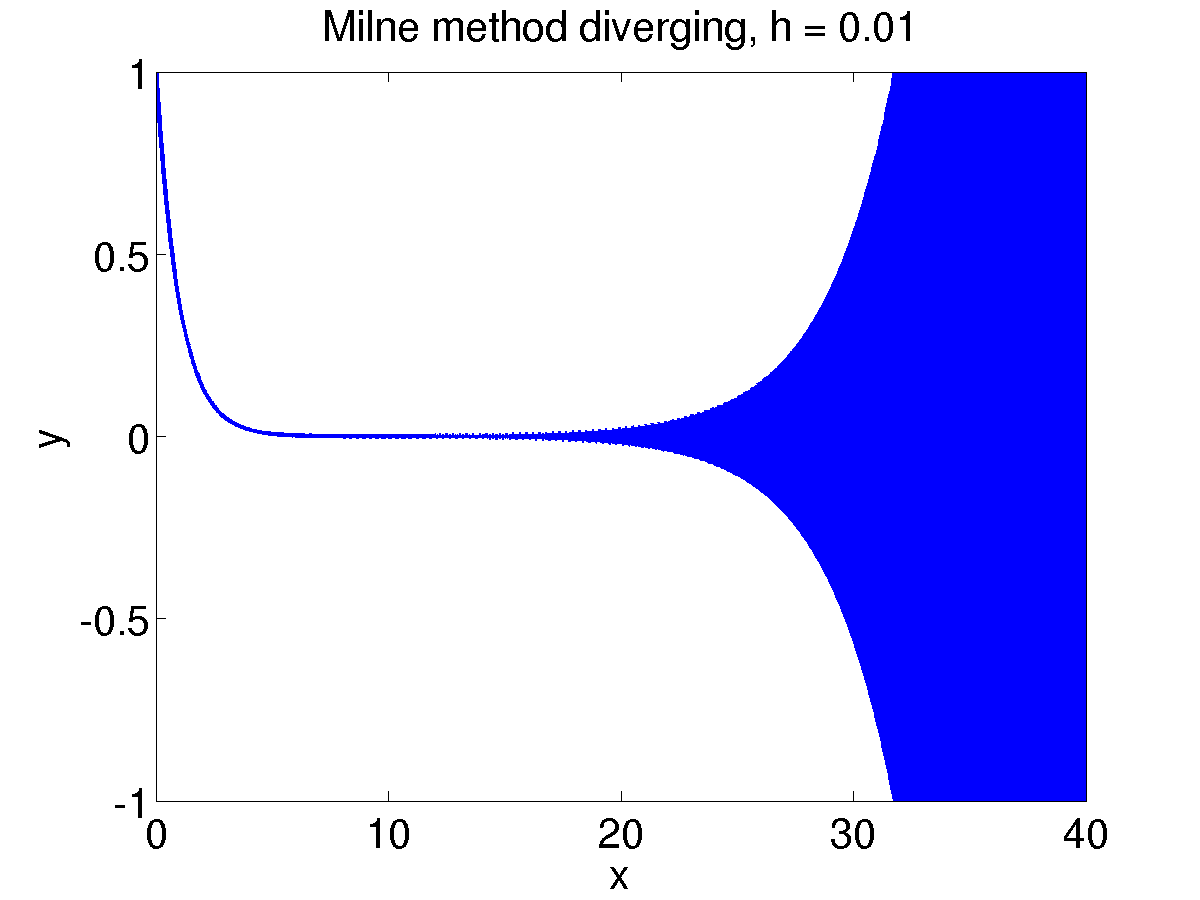
\includegraphics[height=0.5\textheight]{figures/MilneStability1}
          \end{center}
        }
        \only<3|handout:0>
        {
          \begin{center}
            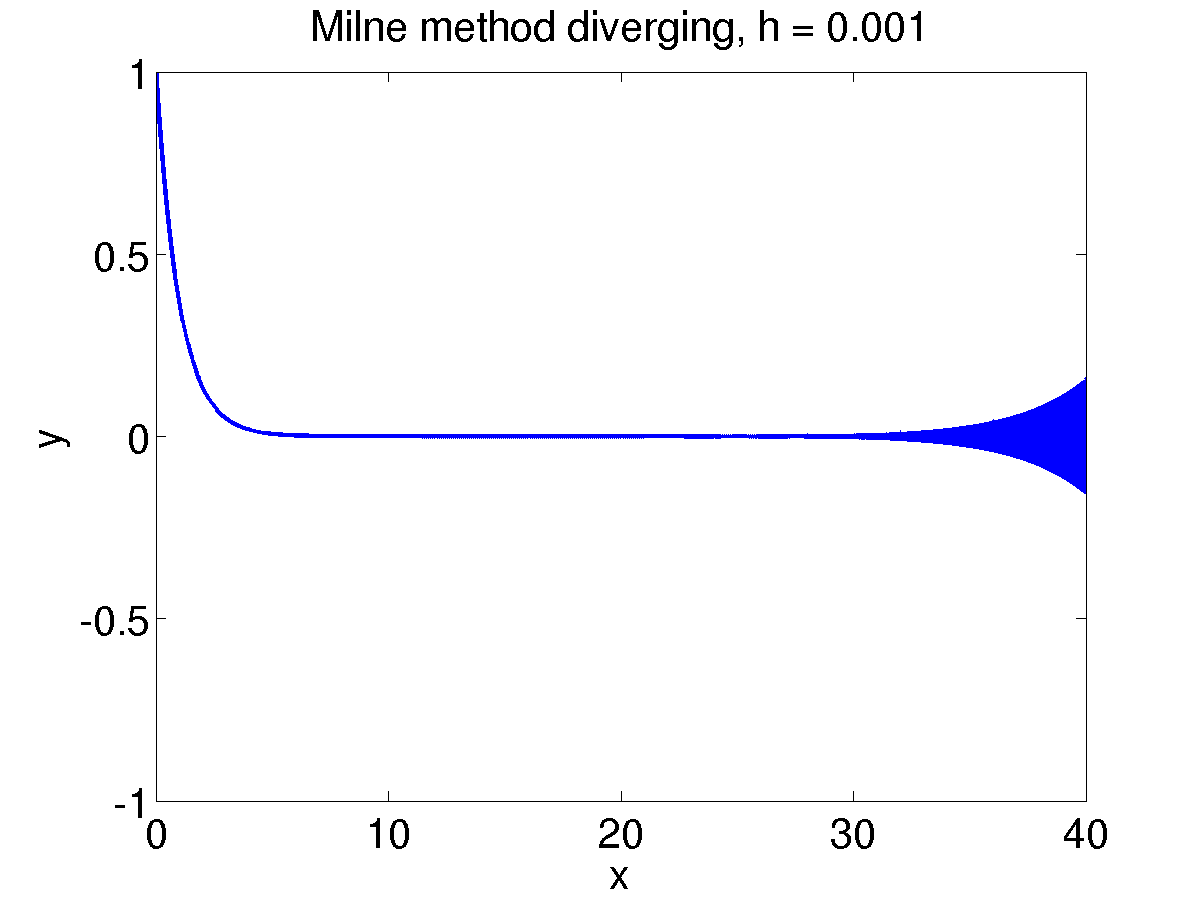
\includegraphics[height=0.5\textheight]{figures/MilneStability2}
          \end{center}
        }
        \only<4|handout:0>
        {
          \begin{center}
            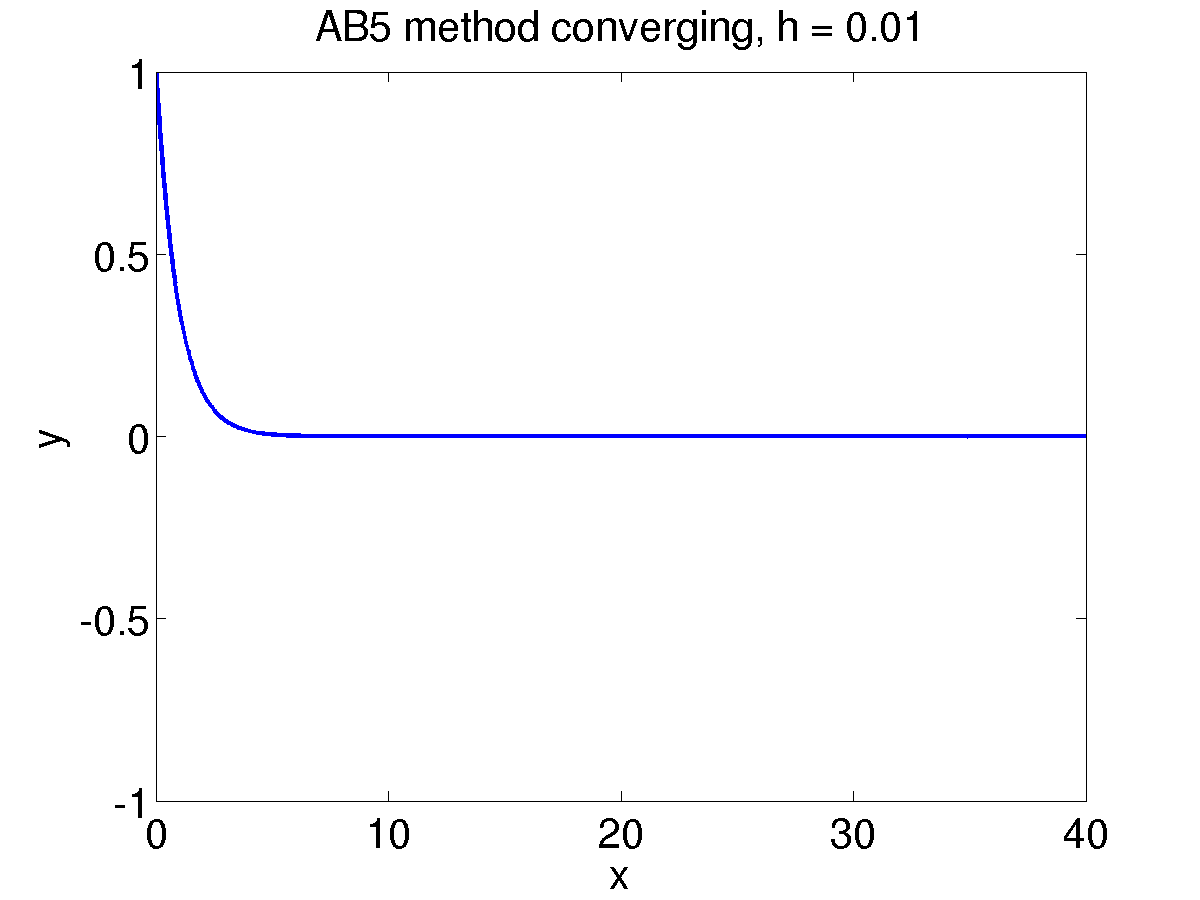
\includegraphics[height=0.5\textheight]{figures/AB5Stability}
          \end{center}
        }
      \end{overlayarea}
    \end{column}
 \end{columns}


\end{frame}



\begin{frame}
  \frametitle{Consistency}

  \emph{Consistency}: the numerical algorithm faithfully represents
  the differential equation. \pause

  \vspace{1ex}

  In other words, in the limit of infinite resolution, $h \rightarrow
  0$, the algorithm should match the differential equation. \pause

  \vspace{1ex}

  To prove consistency use the Taylor expansion of the algorithm. If
  the algorithm is consistent then the expansion at order $h^0 = 1$
  should be the original differential equation. \pause

  \vspace{1ex}

  In practice inconsistent algorithms are useless and will not be seen.

\end{frame}

\begin{frame}
  \frametitle{Stability}

  \emph{Stability}: the method gives bounded results over a
  finite interval. \pause

  \vspace{1ex}

  In other words, for \emph{any} step size $h$ the iteration $\by_n$
  at $x = X$ is \emph{finite}. \pause

  \vspace{1ex}

  Note that we only apply stability criteria to problems where the
  exact solution is finite; the problem
  \begin{equation*}
    y' = \frac{1}{(1-x)^2}
  \end{equation*}
  with solution
  \begin{equation*}
    y(x) = \frac{1}{1-x}
  \end{equation*}
  cannot be considered on intervals including $x = 1$. \pause

  \vspace{1ex}

  Stability is not the only property of an algorithm that we want to
  show, but combined with consistency it does give us everything we
  need.

\end{frame}

\begin{frame}
  \frametitle{Convergence}

  If $y_e(x)$ is the exact solution to the IVP, and $y_h(x)$ the
  numerical solution computed with step size $h$, then a method is
  \emph{convergent} if
  \begin{equation*}
    \lim_{h \rightarrow 0} y_h(x) = y_e(x).
  \end{equation*}
  Convergence is what we want to require of any algorithm. \pause

  \vspace{1ex}

  Convergence is difficult to prove directly. Instead we rely on:

  \vspace{1ex}

  {\bf Theorem}: A multistep method is convergent if and only if it is
  consistent and stable.

\end{frame}

\begin{frame}
  \frametitle{Polynomials for multistep methods}

  \begin{overlayarea}{\textwidth}{0.9\textheight}
    \only<1|handout:1>
    {
      From the $k$-step formula
      \begin{equation*}
        a_k y_{n+1} + a_{k-1} y_n + \dots + a_0 y_{n+1-k} = h \left[ b_k
          f_{n+1} + b_{k-1} f_n + \dots + b_0 f_{n+1-k} \right]
      \end{equation*}
      for multistep methods, define two polynomials
      \begin{align*}
        p(z) & = a_k z^k + \dots + a_1 z + a_0, \\
        q(z) & = b_k z^k + \dots + b_1 z + b_0.
      \end{align*}
    }
    \only<2|handout:2>
    {
      \begin{align*}
        p(z) & = a_k z^k + \dots + a_1 z + a_0, \\
        q(z) & = b_k z^k + \dots + b_1 z + b_0.
      \end{align*}
      Evaluate the \emph{stability} polynomial $p$ and its
      derivative $p'(z)$ at $z=1$:
      \begin{align*}
        p(1) & = \sum_{j=0}^k a_j, \\
        p'(1) & = \sum_{j=0}^k j a_j.
      \end{align*}
    }
    \only<3|handout:3>
    {
      \begin{align*}
        p(z) & = a_k z^k + \dots + a_1 z + a_0, \\
        q(z) & = b_k z^k + \dots + b_1 z + b_0.
      \end{align*}
      \begin{align*}
        p(1) & = \sum_{j=0}^k a_j, \\
        p'(1) & = \sum_{j=0}^k j a_j.
      \end{align*}
      Evaluate the second polynomial $q$ at $z=1$:
      \begin{align*}
        q(1) & = \sum_{j=0}^k b_j.
      \end{align*}
    }
    \only<4|handout:4>
    {
      \begin{align*}
        p(z) & = a_k z^k + \dots + a_1 z + a_0, \\
        q(z) & = b_k z^k + \dots + b_1 z + b_0.
      \end{align*}
      \begin{equation*}
        p(1) = \sum_{j=0}^k a_j, \quad p'(1)  = \sum_{j=0}^k j a_j,
        \quad q(1) = \sum_{j=0}^k b_j.
      \end{equation*}
      In the previous lecture we computed the Taylor expansion using
      the linear functional, showing that for consistency we need
      \begin{align*}
        \sum_{j=0}^k a_j & = p(1) = 0, \\
        \sum_{j=0}^k (j a_j - b_j) & = p'(1) - q(1) = 0.
      \end{align*}
    }
  \end{overlayarea}

\end{frame}

\begin{frame}
  \frametitle{How many solutions...}

  A differential equation has many solutions; initial conditions pick
  out one unique solution.  \pause With non-zero $h$ and finite
  precision, we introduce some error: numerical solution picks up a
  small contribution from other solutions. \pause

  \vspace{1ex}

  Two types of stability are
  \begin{enumerate}
  \item Over a finite interval, say $x \in [0, s]$, the difference
    between the numerical solution and the true solution is
    bounded. \pause
  \item As the number of steps taken is increased the contribution of
    the ``spurious'' solutions tends to zero.
  \end{enumerate} \pause

  Check stability by looking at the roots of the stability polynomial
  \begin{equation*}
    p(z) = \sum_{j=0}^k a_j z^j.
  \end{equation*}

\end{frame}

\begin{frame}
  \frametitle{Why the roots of the polynomial?}

  For stability the numerical solution must remain finite. \pause
  Consider the case $f(x, y(x)) = 0$.  Algorithm becomes
  \begin{equation*}
    \sum_{j=0}^k a_j y_{n+1-j} = 0.
  \end{equation*} \pause

  \vspace{1ex}

  Difference equation has $k$ solutions of form $A z^n$: $A$
  depends on initial data, $z$ depends on algorithm. \pause To
  converge, require $|z| < 1$. \pause

  \vspace{1ex}

  To find solutions substitute in $A z^n$, finding
  \begin{equation*}
    A z^{n+1-k} \sum_{j=0}^k a_j z^j \propto p(z).
  \end{equation*} \pause
  Therefore the size of the roots of $p(z)$ are crucial for stability.

\end{frame}



\begin{frame}
  \frametitle{Stability conditions}

  Write roots of stability polynomial $p$ as $\{r_j\}$. Two
  conditions:
  \begin{enumerate}
  \item If $ | r_j | \leq 1$ for all of the $k$ roots, \emph{and} any
    root with $|r_j| = 1$ is simple (i.e.\ is not repeated), then the
    \emph{root condition} is satisfied. \pause
  \item If $r_0 = 1$ and $ | r_j | < 1$ for all of the other $k-1$
    roots then the \emph{strong} root condition is satisfied.
  \end{enumerate} \pause

  \vspace{1ex}

  Either condition is sufficient for \emph{weak} stability. To ensure
  correct \emph{long term} integrations, need both stability
  (guaranteed by root condition) and \emph{relative} stability (given
  by strong root condition).

\end{frame}

\begin{frame}
  \frametitle{Example}

  \begin{overlayarea}{\textwidth}{0.9\textheight}
    \only<1|handout:1>
    {
      The Milne method
      \begin{equation*}
        y_{n+1} - y_{n-1} = \frac{h}{3} \left( f_{n+1} + 4 f_{n} + f_{n-1} \right)
      \end{equation*}
      is a $k$-step method with coefficients
    }
    \begin{align*}
      a_0 & = -1, & a_1 & = 0, & a_2 & = 1, \\
      b_0 & = 1/3, & b_1 & = 4/3, & b_2 & = 1/3.
    \end{align*}
    \only<2-3|handout:1>
    {
      Consistency shown when it was proved to have
      order 4. Can check:
    }
    \only<2-5|handout:1-2>
    {
      \begin{align*}
        &&    p(z) & = \sum_{j=0}^k a_j z^j & q(z) & = \sum_{j=0}^k b_j z^j \\
        && & = z^2 - 1 && = \tfrac{1}{3} \left( z^2 + 4 z + 1 \right)
        \\
        \Rightarrow && p'(z) & = 2 z
      \end{align*}
    }
    \only<3|handout:0>
    {
      and hence
      \begin{equation*}
        p(1)  = 0, \quad
        p'(1)  = 2 = q(1).
      \end{equation*}
    }
    \only<4-5|handout:2>
    {
      Roots of the stability polynomial are $r_j = \pm 1$: Milne's
      method is only weakly stable.
    }
    \only<5|handout:2>
    {
      Expect the method to converge, but spurious solutions may
      dominate for long integrations.
    }
  \end{overlayarea}
\end{frame}

\begin{frame}
  \frametitle{Example: 2}

  \begin{columns}
    \begin{column}{0.5\textwidth}
      Integrate
      \begin{equation*}
        y'(x) = -y, \quad y(0) = 1
      \end{equation*}
      with solution $y = \exp(- y(0) x)$. \pause

      \vspace{1ex}

      As the Milne method is not strongly stable we see
      divergence. \pause

      \vspace{1ex}

      As the method is weakly stable, we see that the time the
      divergence sets in increases with better resolution.
    \end{column}
    \begin{column}{0.5\textwidth}
      \begin{overlayarea}{\textwidth}{0.6\textheight}
        \only<2|handout:0>
        {
          \begin{center}
            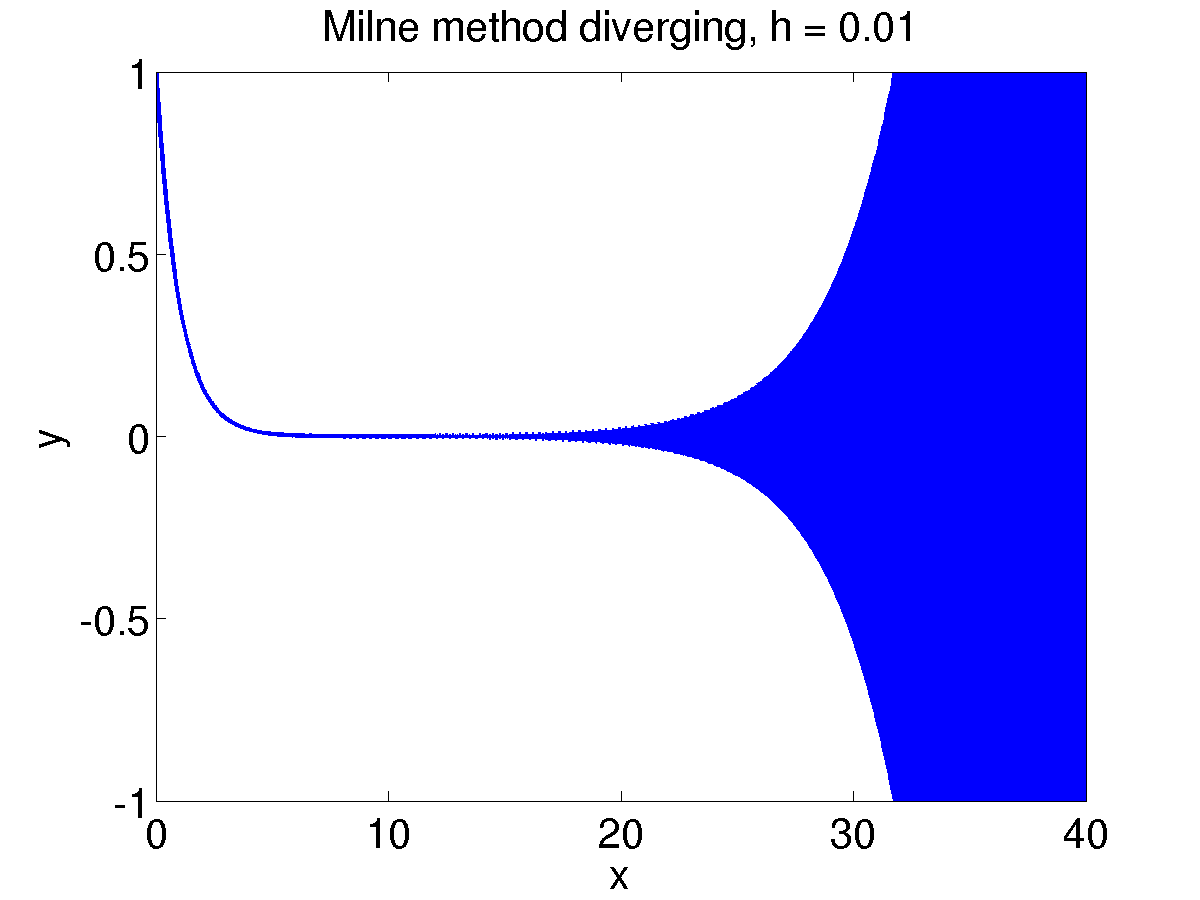
\includegraphics[height=0.5\textheight]{figures/MilneStability1}
          \end{center}
        }
        \only<3>
        {
          \begin{center}
            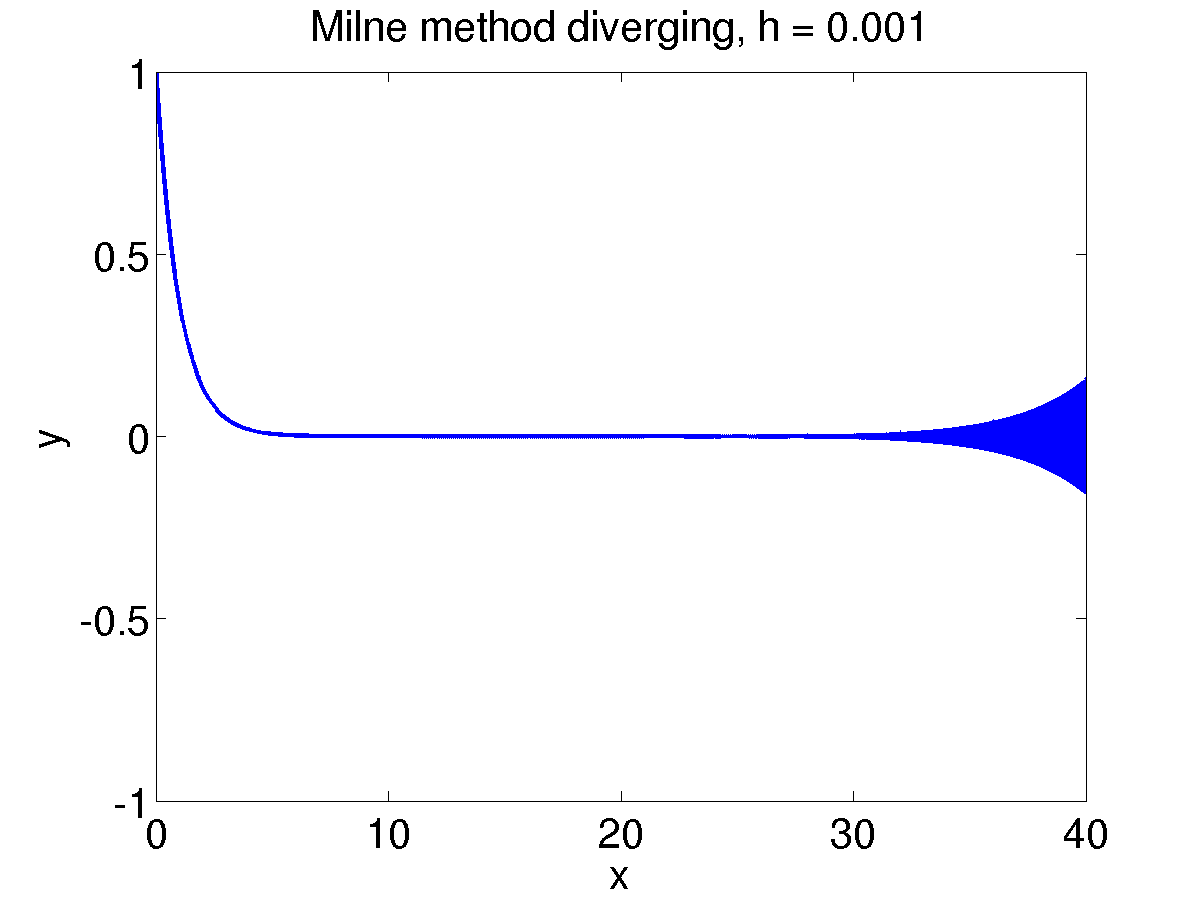
\includegraphics[height=0.5\textheight]{figures/MilneStability2}
          \end{center}
        }
      \end{overlayarea}
    \end{column}
 \end{columns}

\end{frame}

\section{Summary}

\subsection{Summary}

\begin{frame}
  \frametitle{Summary}

  \begin{itemize}
  \item Convergence to the correct solution is the requirement for any
    algorithm.
  \item For differential equations the algorithm must be
    \emph{consistent} and \emph{stable}; in many cases this is
    sufficient for convergence.
  \item For multistep methods we define two polynomials $p$ (the
    stability polynomial) and $q$ depending on the coefficients in the
    $k$-step formula.
  \item Consistency is given by two simple relations between the
    polynomials (and derivatives) evaluated at $z=1$; it is equivalent
    to proving that the lowest order local truncation error terms
    vanish.
  \item Stability is shown by checking the modulus of the roots of $p$:
    \begin{enumerate}
    \item If all roots are $|r_j|<1$ (except $r_0=1$) then we have
      relative stability.
    \item If we do not have relative stability, but all $|r_j| \leq
      1$, then we have \emph{weak} stability which may not be
      sufficient for good long term integrations.
    \end{enumerate}
  \end{itemize}

\end{frame}

\end{document}



%%% Local Variables:
%%% mode: latex
%%% TeX-master: t
%%% End:
